\documentclass[12pt]{extarticle}
\usepackage[utf8]{inputenc}
\usepackage[margin =0.5in]{geometry}
\usepackage[inline]{enumitem}  
\usepackage{tabularx}
\usepackage{amsmath}
\usepackage{graphicx}
\usepackage{hyperref}
\usepackage{booktabs, multirow} % for borders and merged ranges
\usepackage{soul}% for underlines
\usepackage[table]{xcolor} % for cell colors
\usepackage{changepage,threeparttable} % for wide tables

\graphicspath{ {./images/} }


\author{Name: Sean Balbale}
\date{December 2022}
\title{AP Physics: The Simple Pendulum Lab Report}

\begin{document}
\section*{AP Physics: The Simple Pendulum Lab Report}
\begin{enumerate*}[label={}]
    \item Name: Sean Balbale
    \item December, 2022
\end{enumerate*}
\pagebreak
\tableofcontents
\pagebreak

\section{Lab Setup and Procedure:}
\subsection{Setup:}
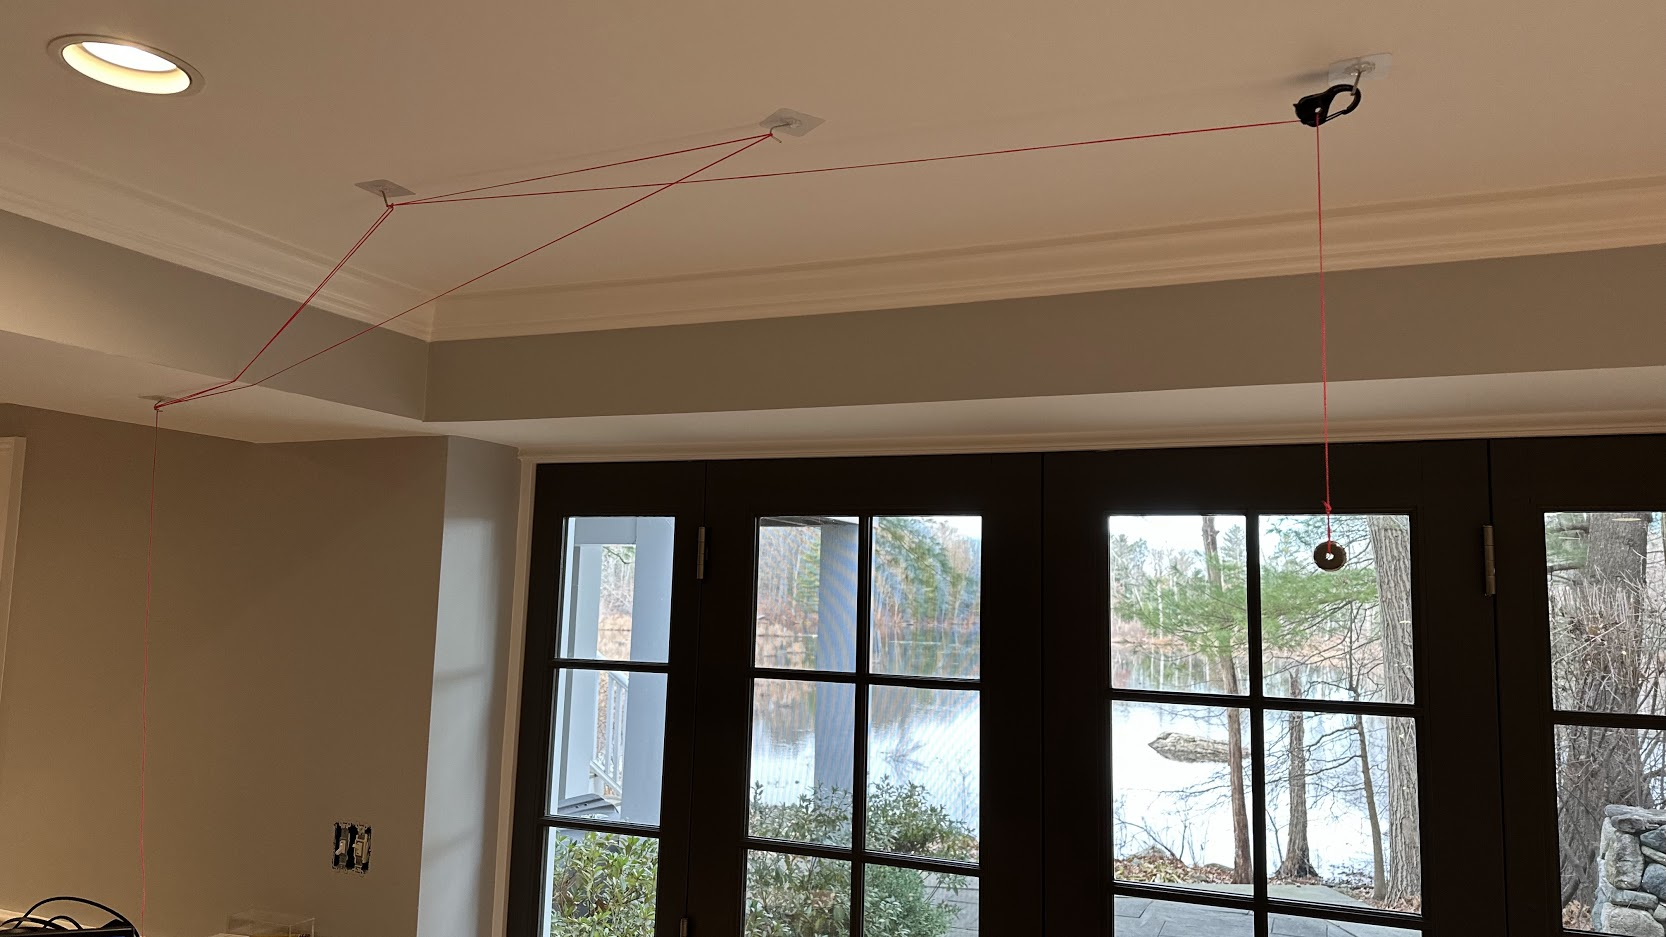
\includegraphics[scale=0.25]{Still Frame Lab Setup.png}
\subsection{Procedure:}
I created a pendulum from mason twine which is a light weight nylon string. I used a circular piece of metal as the bob.
I hung the pendulum from the ceiling and let it swing freely. I then recorded the time it took for the pendulum to swing for at least $15$ periods.
With the multiple periods I used $5$ of them to calculate the average period for a certain length of string.
I repeated this process $8$ times for string lengths between $0.5$ and $2.25$ meters and recorded the data in the table below.

\pagebreak
\section{Data and Graphs:}
\begin{table}[!htp]\centering
    \caption{Raw Time Data}\label{tab: }
    \scriptsize
    \begin{tabular}{lrrrrrrrrrrrrrrrr}\toprule
        trial: & start & end  & period 1 & start & end   & period 2 & start & end   & period 3 & start & end   & period 4 & start & end   & period 5 \\\cmidrule{1-16}
        1      & 6.63  & 8.05 & 1.42     & 8.05  & 9.46  & 1.41     & 9.46  & 10.88 & 1.42     & 10.88 & 12.29 & 1.41     & 12.29 & 13.7  & 1.41     \\\cmidrule{1-16}
        2      & 3.57  & 5.31 & 1.74     & 5.31  & 7.04  & 1.73     & 7.04  & 8.78  & 1.74     & 8.78  & 10.52 & 1.74     & 10.52 & 12.25 & 1.73     \\\cmidrule{1-16}
        3      & 7.12  & 9.12 & 2        & 9.12  & 11.09 & 1.97     & 11.09 & 13.09 & 2        & 13.09 & 15.06 & 1.97     & 15.06 & 17.06 & 2        \\\cmidrule{1-16}
        4      & 3.63  & 5.87 & 2.24     & 5.87  & 8.15  & 2.28     & 8.15  & 10.36 & 2.21     & 10.36 & 12.63 & 2.27     & 12.63 & 14.85 & 2.22     \\\cmidrule{1-16}
        5      & 4.84  & 7.27 & 2.43     & 7.27  & 9.72  & 2.45     & 9.72  & 12.15 & 2.43     & 12.15 & 14.57 & 2.42     & 14.57 & 17.03 & 2.46     \\\cmidrule{1-16}
        6      & 3.21  & 5.81 & 2.6      & 5.81  & 8.42  & 2.61     & 8.42  & 11.12 & 2.7      & 11.12 & 13.72 & 2.6      & 13.72 & 16.48 & 2.76     \\\cmidrule{1-16}
        7      & 4.72  & 7.55 & 2.83     & 7.55  & 10.48 & 2.93     & 10.48 & 13.21 & 2.73     & 13.21 & 16.05 & 2.84     & 16.05 & 18.9  & 2.85     \\\cmidrule{1-16}
        8      & 4.84  & 7.85 & 3.01     & 7.85  & 10.86 & 3.01     & 10.86 & 13.86 & 3        & 13.86 & 16.87 & 3.01     & 16.87 & 19.88 & 3.01     \\\midrule
        \bottomrule
    \end{tabular}
\end{table}
\begin{table}[!htp]\centering
    \caption{Length and Periods}\label{tab: }
    \scriptsize
    \begin{tabular}{lrrrrr}\toprule
        trial & length (m) & period (s) & log(L)   & log(T)  \\\cmidrule{1-5}
        1     & 0.5        & 1.414      & -0.30103 & 0.15045 \\\cmidrule{1-5}
        2     & 0.75       & 1.736      & -0.12494 & 0.23955 \\\cmidrule{1-5}
        3     & 1          & 1.988      & 0        & 0.29842 \\\cmidrule{1-5}
        4     & 1.25       & 2.244      & 0.09691  & 0.35102 \\\cmidrule{1-5}
        5     & 1.5        & 2.438      & 0.17609  & 0.38703 \\\cmidrule{1-5}
        6     & 1.75       & 2.654      & 0.24304  & 0.4239  \\\cmidrule{1-5}
        7     & 2          & 2.836      & 0.30103  & 0.45271 \\\cmidrule{1-5}
        8     & 2.25       & 3.008      & 0.35218  & 0.47828 \\\midrule
        \bottomrule
    \end{tabular}
    \end{tabular}
\end{table}

\begin{figure}[!htp]
    \centering
    \caption{Log(T) vs. Log(L)}\label{fig: }
    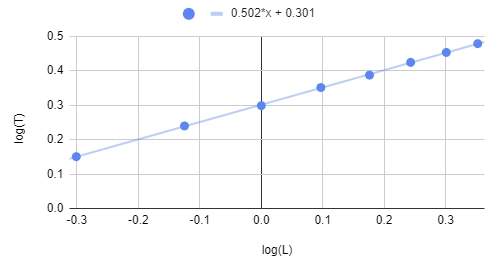
\includegraphics[scale=1]{Log(t)vslog(L).png}
\end{figure}


\pagebreak
\section{Diagram and Calculations:}
\subsection{Variables:}
period: $T$
\\ length of string: $L$
\\ gravity: $g$
\\\subsection{Equations:}
\begin{equation}
    T = cL^p
\end{equation}
\begin{equation}
    T = 2*\pi*\sqrt{\frac{L}{g}}
\end{equation}
\begin{equation}
    g=(\frac{2 \pi}{c})^2
\end{equation}

\subsection{Calculations:}
\textbf{Now we can calculate the values of $p$ and $c$:}
\\By taking the log of both sides of equation 1 we get:
\begin{equation}
    log(T) = plog(L) + log(c)
\end{equation}
\\Using this equation it becomes clear that the slope of the graph of log(T) vs. log(L) is equal to $p$, and the y-intercept is equal to $log(c)$.
\\The slope of the graph is $0.516$ and the y-intercept is $0.301$.
\\Now by reversing the log function for $log(c)$ we get the value of $c$:
\begin{equation}
    c = 10^{0.301} = 2.000
\end{equation}
\\Now that we know that $p$ is equal to $0.516$ and $c$ is equal to $2.000$ we can fill out equation 1:
\begin{equation}
    T = 2.00L^{0.516}
\end{equation}
Let's see how accurate equation 6 is by plugging in a value of $L$ from the table and testing it against equation 2:
\begin{equation}
    T_{calculated} = 2.00(0.5)^{0.516} = 1.414
\end{equation}
\begin{equation}
    T_{actual} = 2*\pi*\sqrt{\frac{0.5}{9.81}} = 1.419
\end{equation}
Lets calculate the relative percent error of the calculated value of $T$:
\\$T_{actual} = 1.419 s$
    \\$T_{calculated} = 1.414 s$
\\$T_{error} = \frac{|T_{actual} - T_{calculated}|}{T_{actual}} \times 100 = \frac{|1.419 - 1.414|}{1.419} \times 100  = 0.298 \%$
    \\Using the found value of $c$ we can calculate the value of $g$ by using equation 3:
    \begin{equation}
        g = (\frac{2 \pi}{2.00})^2 = 9.868
    \end{equation}
    Lets calculate the relative percent error of the calculated value of $g$:
    \\$g_{actual} = 9.81 m/s^2$
\\$g_{calculated} = 9.868 m/s^2$
    \\$g_{error} = \frac{|g_{actual} - g_{calculated}|}{g_{actual}} \times 100 = \frac{|9.81 - 9.868|}{9.81} \times 100  = 0.594 \%$
\pagebreak

\section{Closing thoughts:}
The relative percent error of the calculated value of $T$ is 0.298\%. This is a very small error, so the constants $c$ and $p$ were very close to their actual values.
Despite the slight error in the calculated value of $T$, the relative percent error of the calculated value of $g$ is 0.594\%. This is a larger error than the error of the calculated value of $T$.
Even though this error is larger, it is still relatively small, so the experiment was still very accurate.
Despite this accurate calculation, many things could have gone wrong. For example, the string could have been longer or shorter than the lengths we measured.
This would have caused the pendulum's period to be different from what it should have been. In addition, the way that I attached the string to the ceiling had the potential to swing a bit.
This would have resulted in a circular motion which could have thrown off the pendulum's period.
I am pleased with the experiment's results, as the calculated value of $g$ is very close to the actual value of $g$, and the equation $T = 2.00L^{0.516}$ does an excellent job of predicting the period of a pendulum with a given length $L$.
\end{document}


